\begin{remark}
这部分是我们调研的全部内容的整理与总结,包括但不限于我们在下一部分\ref{chap:method}中着重讨论的APSI技术,因此这部分篇幅较长。
\end{remark}

\section{Background}
\subsection{Private set intersection (PSI)}
私有集合求交 (PSI) 是一种安全多方计算的密码学技术,它允许各自持有集合的两方比较这些集合的加密版本以计算交集。在这种情况下,除了交集中的元素外,任何一方都不会向交易对手透露任何信息。形式化地,两方各自拥有集合 $S=\{s_1,s_2,...,s_n\}$ 和 $S'=\{s_1',s_2',...,s_n'\}$,其中 $s_i,s_i'\in\{0,1\}^\sigma$ 并且假设 $S,S'$ 中各自都没有重复的元素。目标:各方计算 $I=S\cap S'$,不泄露除了 $I$ 之外的任何信息。

\subsection{Adversary model}
\noindent\textbf{Semi-honest Model}:完全按照密码学的协议执行,但会尽可能尝试从收到的信息中获取额外的信息。

\noindent\textbf{Malicious Model}:可以不严格按照密码学的协议执行,可以做任何事情来达到获取额外信息的目的。

\subsection{Cuckoo hashing}\cite{charlesCuckoo}
布谷鸟哈希最早于2001年由Rasmus Pagh 和Flemming Friche Rodler 提出。该哈希方法是为了解决哈希冲突的问题而提出,利用较少计算换取了较大空间。

\subsubsection{插入逻辑}
\noindent 设插入的值为x:
\begin{enumerate}
    \item 若值x已在哈希表中则直接返回。
    \item 若插入后哈希表空间不足则先进行扩容,再rehash,然后进行3、4、5。
    \item 用哈希函数$h_1(x)$计算出x应该插入的桶下标$i_1$,若bucket[$i_1$]空则直接插入。
    \item 若bucket[$i_1$]非空,则将bucket[$i_1$]中的老值$x_{old}$踢开,并用哈希函数$h_2(x_{old})$寻找$x_{old}$应该填的下一个位置。
    \item 设插入值为$x_{old}$重复2,直到达到最大循环次数(插入失败),或者被踢开的值都找到了新的位置(插入成功)。
\end{enumerate}

\subsubsection{查找逻辑}
使用两个哈希函数$h_1(x)$和$h_2(x)$计算需要查找的值有可能在的两个桶,若没有匹配则查找失败,否则查找成功。

\subsubsection{运行时间分析}
插入的最坏循环次数是常数,插入的摊还时间复杂度为$O(1)$。
当哈希表空间不足时需要进行扩容操作,对于n次插入,需要$O(\log n)$次扩容,每次需要进行重新哈希,大小分别为$n,n/2,···,n/2^{O(\log n)}$,所需要的时间为$O(n+n/2+···+n/2^{O(\log n)})<O(n+n/2+n/4···)=O(n)$。因此对于n个插入操作扩容的摊还时间为$O(1)$。

 1.插入循环分析:\\
设插入x会驱逐y,y插入到新位置会驱逐z···\\
设这个序列$x_1=x,x_2=y,x_3=z···$为无巢序列。\\
情况1:无巢序列没有重复的元素,即$x_1\ne x_2\ne x_3···$,这种情况下经过O(1)时间即可结束插入。\\
情况2:无巢序列中有重复元素:这里假设$x_i$在位置$x_j$被第二次移除,i$<$j,则此时若此位置是由$h_1(x)$所得的,则用$h_2(x)$计算其下个位置,反之亦然。这种情况下,插入过程会回溯$x_i$前面的一系列键,从$x_i=x_j$开始,$x_{i-1}=x_{j+1}···$,直到$x_1=x_{j+i-1}$,这些键都被回退到x未被插入之前的位置(对应图3.1中step9-12),然后把x放到位置$h_2(x)$,这样插入过程就会继续,直到某个$x_l$被插入一个空的位置,或者$x_l$再次与前面的某个键相同,如果最终陷入死循环,则需要进行重新哈
\begin{figure}[h]
    \centering
    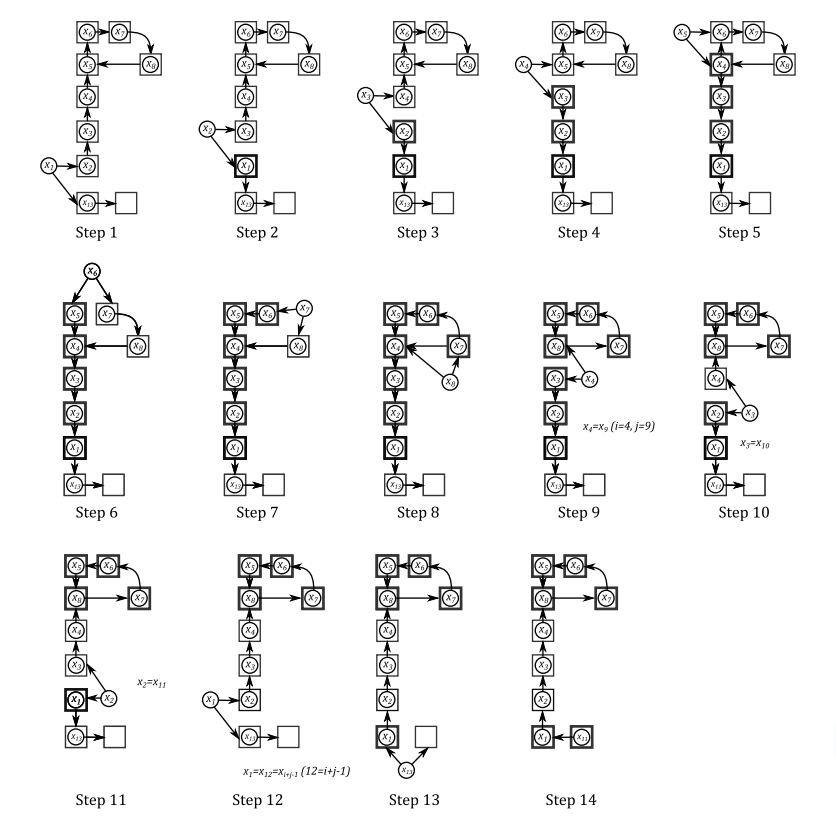
\includegraphics[width=17cm]{cuckoo hashing}
    \caption{cuckoo hashing}
    \label{fig:cuckoo hashing}
\end{figure}
为了进行插入的时间复杂度分析,需要使用如下引理:
\begin{lemma}
假设在某步p, x的插入过程产生一个序列$x_1=x,x_2,···,x_p$的无巢键,其中还没有形成闭环(即死循环)。在$x_1,···,x_p$中,存在长度为$l\ge p/3$的连续子序列$x_q,x_{q + 1},···,x_{q + l−1}$其中的无巢键各不相同,且其中$x_q = x_1 = x$。
\end{lemma}
2.时间复杂度分析:\\
考虑插入过程产生长度k$\le$2MaxLoop的无巢键序列,会产生以下三种情况:\\
情况1:哈希函数不是随机选则的。这种情况发生的概率为$O(1/n^2)$。\\
情况2:插入过程还未陷入死循环。这种情况发生的概率为$O(2(1+\epsilon)^{-\frac{k-1}{3}+1})$,其中哈希表大小r$\ge (1+\epsilon)n$。\\
情况3:插入过程已经陷入死循环。这种情况发生的概率为$O(1/n^2)$。\\

\begin{proof}
情况2:当插入过程未陷入死循环时,根据引理1,有一组长度为$v=\lceil k/3 \rceil$的连续不相等无巢键序列$b_1=x,b_2,···,b_v$。根据插入操作的方法,连续的序列的哈希函数值相等。而哈希函数是随机选取的,键的值域为$0,1,···,r-1$,所以两个哈希函数的值相等的概率为$1/r^2$,此序列能够满足条件的概率为$1/r^{v-1}$。同时,有不多于$n^{v-1}$种产生连续不相等无巢键序列的情况,因此产生此种序列的概率为:
  \[2n^{v-1}r^{-(v-1)}=2(r/n)^{-(v-1)} \le 2(1+\epsilon)^{-k/3+1}\]
这里使用了条件r$\ge (1+\epsilon)n$。\\
其他证明略。
\end{proof}
因此,可以计算出一个插入循环产生的无巢键数为:
\[1+\sum^{2MaxLoop}_{k=2}[2(1+\epsilon)^{-k/3+1}+O(1/{n^2})]\le 1+O(MaxLoop/n^2)+2\sum^{inf}_{k=0}(1+\epsilon)^{-k/3}=O(1)+\frac{O(1)}{1-(1+\epsilon)^{-1/3}}=O(1)\]
因此插入迭代次数为常数,时间复杂度为常数。
\subsection{Oblivious Transfer}
 OT协议可以让发送者在不知道接收者需要哪些信息的情况下,互相交换信息。一般来说,OT协议被用来在远程计算中共享私密数据,以确保这些数据只能被授权用户获得.\\
OT协议的主要思想是发送方能够向接收方发送多个消息,但仅有其中一条消息与接收方真正需要的消息有关。发送方无法确定实际的情况,因此不会泄露再多信息.\\
OT协议可以追溯到1981年Rabin提出的方案\cite{rabin1981exchange},其用途是在密钥交换中保护计算机所处网络的连续性。后来,OT协议被证明与多方计算,安全多方计算(SMPC)和私有信息检索(PIR)等密码学问题密切相关。更完善的不经意传输形式被称为"1–2 oblivious transfer"或 "1 out of 2 oblivious transfer",即发送方向接收方发送两个消息,接收方只能选择其中一个消息,同时而言,发送方对于接收方到底选择了哪一个消息一无所知,由Shimon Even、Oded Goldreich和Abraham Lempel开发\cite{even1985randomized},以建立用于安全多方计算的协议。后续"1–n oblivious transfer"的具体方案也被提出.\\

\begin{enumerate}
    
 \item  第一种OT由Rabin于1981年\cite{rabin1981exchange}提出:\\
其假设$Alice$有秘密$S_A$,$Bob$有秘密$S_B$,并且秘密为单比特,$Alice$ 和 $Bob$ 想要交换秘密,要求两方都有可能得到秘密并且秘密拥有方不知道对方是否得到秘密:
    \begin{enumerate}
    \item  $Alice$随机选取两个大素数$p,q$。并计算得到$one-time-  key ~~ n_ {A} $ , 然后将 $ n_ {A} $ 发
送给$Bob$。
   \item  $Bob$随机选取一个数x,要求$x <  n_ {A} $ ,计算$ c \equiv  x^ {2}  mod ~n_ {A} $ ,然后将 $c$ 和私钥加密的 $x$ 发送给$Alice$。
   \item  $Alice$找到一个 $ x_ {1} $ 使得 $ x_ {1}^ {2}  \equiv cmod(  n_ {A} )$ ,发送 $ x_ {1} $ 给$Bob$。
   \item  $Bob$计算 $ gcd(x-  x_ {1}  ,  n_ {A}  )=d $, 此时有 $P(d = q\ or\ d = q)=  \frac {1}{2} $ 。
   \item  $Bob$根据计算  $ v_ {B} $ = $ \begin{cases}0,if(x-x_{1},n_{A})=p~or~q,\\1,otherwise.\end{cases} $ 
    接着计算 $ \varepsilon _ {B} $ = $ v_ {B} $ $ \oplus $ $ S_ {B} $ 然后将 $ \varepsilon _ {B} $ 发送给$Alice$.
    \end{enumerate}
    \noindent 这是$Alice$获得$Bob$的秘密 $ S_ {B} $ 的过程,可以得出$Alice$得到 $ S_ {B} $ 的概率为 $ \frac {1}{2} $ 。$Bob$获得 $ S_ {A} $ 的过程依然是上述步骤, 只不过是将$Alice$和$Bob$角色互换。\\
 \item  OT based on DH\cite{naor2001efficient}  \\
   有如下假设
   \begin{enumerate}
    \item  $Alice$拥有值 $ v_ {0} $ , $ v_ {1} $ 和密钥$s$, $ r_ {0} $ , $ r_ {1} $ 
    \item  $Bob$拥有值 $i \in {0,1} $ 和密钥$k$。$Bob$想获得 $ v_ {i} $ 
    \item  $Alice $和$Bob$ 事先统一$g  \in  Z_p$, 其中$g$是大整数, $p$是大素数
   \end{enumerate} 
    \noindent 具体过程为:

    \begin{enumerate}
    \item $Alice  \rightarrow  Bob:  g^ {s} $ .
    \item $Bob$ 基于 $i$ 生成 $$L_i  =  \begin{cases} g^k  &,  if~ i = 0 ,\\ g^{s-k} &,if~i=1.\end{cases} $$
    \item $Bob$ $ \rightarrow $ $Alice$: $ L_ {i} $ 
    \item $Alice$生成 $ C_ {0} $ , $ C_ {1} $\\
       $ C_ {0}  =(g^{r_0} ,(L_i)^{r_0} \oplus   v_ {0} )$ \\
       $ C_ {1}  =(g^{r_1} ,(g^s / L_i)^{r_1} \oplus   v_ {1} )$ )
    \item  $Alice$ $ \rightarrow $ Bob: $ C_0, C_1 $ 
    \item  $Bob$解密 $ v_ {i} $ 
        \begin{enumerate}    
        \item  $case ~i=0$
            \begin{enumerate}            
            \item  $Bob$ 可以通过如下方式解密获得 $ v_ {0} $ :\\
               $ C_ {0} $ $ [0]^ {k} $ $ \oplus $ $ C_ {0} $ [1]= $ (g^ {r_ {0}})^ {k} $ $ \oplus $ $ (L_ {i})^ {r_ {0}} $ $ \oplus $ $ v_ {0} $ = $ (g^ {r_ {0}})^ {k} $ $ \oplus $ $ (g^ {k})^ {r_ {0}} $ $ \oplus $ $v_0=v_0$
            \item  $Bob$无法获得 $ v_ {1} $ 因为 $ C_ {1}  [1]=  (g^ {s}/L_{i})^ {r_ {1}} $ $ \oplus $ $ v_ {1} $ = $ g^ {(s-k)r1} $ $ \oplus $ $ v_ {1} $ 而$Bob$不知道$s$, $ r_ {1} $ 
            \end{enumerate}
        \item  $case~ i=1$
            \begin{enumerate}
           \item  类似地, $Bob$ 通过如下方式解密获得 $ v_ {1} $ :\\
            $ C_ {1} $ $ [0]^ {k} $ $ \oplus $ $ C_ {1}  [1]=  (g^ {r1})^ {k} $ $ \oplus $ $ (g^ {s}/L_ {i})^ {r_ {1}} $ $ \oplus $ $ v_ {1} $ = $ (g^ {r_ {1}})^ {k} $ $ \oplus $ $ (g^ {k})^ {r_ {1}} $ $ \oplus $ $ v_ {1} $ = $ v_ {1} $ 
           \item  $ Bob $ 无法获得 $ v_ {0} $ 因为 $ C_ {0}  [1]=  (L_ {i})^ {r0} $ $ \oplus $ $ v_ {0} $ = $ g^ {(s-k)r0} $ $ \oplus $ $ v_ {0} $ 而$Bob$不知道$s,r_0$
           \end{enumerate}
        \item  因此,$Bob$只能解密 $ v_ {i} $ 而不能解密 $ v_ {1-i} $ \\
        \end{enumerate}
    \end{enumerate}
 \item  OT based on RSA\cite{OTRSA} \\
    Even、Goldreich 和 Lempel 的协议可以使用RSA加密方案来实现,如下:
    \begin{enumerate}
    \item  $Alice$拥有消息 $ m_ {0} $ , $ m_ {1} $ , 并其中一个发送给$Bob$。$Bob$不想让$Alice$知道他收到了哪一个.
    \item  $Alice$ 生成一个 RSA 密钥对,包括模数N,公有指数e和私有指数d.
    \item  $Alice$还生成了两个随机值$x_{0},x_{1}$并将它们与模数N和指数e一起发送给$Bob$
    \item  $Bob$选择 $b\in \{0,1\}$并生成随机数 $k$ ; 随后计算$v = (x_b + k^e) mod~ N$,并将 $v$ 发送给$Alice$.
    \item  $Alice$计算$k_0 = (v - x_0)^d ~mod~N $ 和 $k_1 = (v - x_1)^d ~mod~N $; 于是$k_0$ 和 $k_1$ 其中之一是$k$, 但$Alice$并不知道是哪一个.
    \item  $Alice$计算$m_0' = m_0 + k_0$ 和$m_1' = m_1 + k_1$, 将其发送给$Bob$.
    \item  $Bob$计算$m_b = m_b' - k$, 于是$Bob$获得了$Alice$发送的消息$m_b$.
    \end{enumerate}
\end{enumerate}

\newpage

\subsection{Garbled Circuits}
\noindent 混淆电路协议分为四个部分。
\begin{enumerate}

\item Alice 生成混淆电路\\
生成过程主要分四步:
\begin{enumerate}
\item Alice 对电路中的每一线路(Wire)进行标注。如下图所示,Alice 一共标注了七条线路,包括模块的输入输出 $W_{a0}$,$W_{b0}$,$W_{c0}$,$W_{c1}$
,和模块内的中间结果 $W_{d}$,$W_{e}$,$W_{f}$。对于每一条线路 $W_{i}$,Alice 生成两个长度为 k的字符串 $X^0_{i}$,$X^1_{i}$。这两个字符串分别对应逻辑上的 0 和 1。这些生成的标注会在 Step 2 有选择性地发给 Bob,但 Bob 并不知道 $X^0_{i}$,$X^1_{i}$
 对应的逻辑值。
 
\begin{figure}[h]
    \centering
    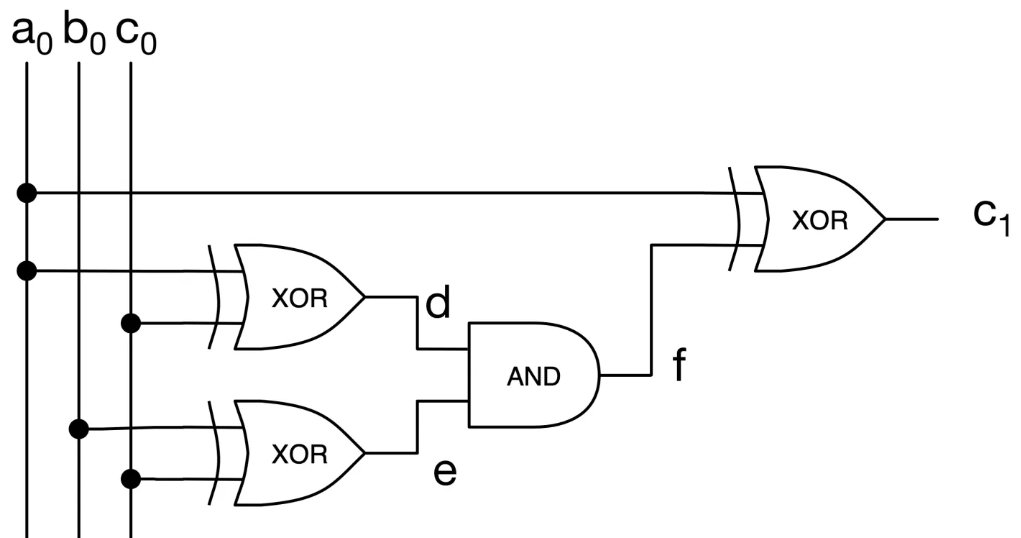
\includegraphics[width=15cm]{circuit.png}
    \caption{circuit}
    \label{fig:circuit}
\end{figure}
\item Alice 对电路中的每一个逻辑门的 Truth Table 用 $X^0_{i}$,$X^1_{i}$
进行替换,由 $X^0_{i}$替换 0,由 $X^1_{i}$替换 1.
 \item Alice 对每一个替换后的 Truth Table 的输出进行两次对称密匙加密(即加密和解密的密匙相同),加密的密匙是 Truth Table 对应行的两个输入。比如 Truth Table 的第一行是 $X^0_{a0}$,$X^0_{c0}$,$X^0_{d}$,我们就用 $X^0_{a0}$,$X^0_{c0}$加密 $X^0_{d}$生成 Enc($X^0_{a0}$,$X^0_{c0}$){$X^0_{d}$}
 。
\item Alice 对第三步加密过后的 Truth Table 的行打乱得到 Garbled Table。所以 Garbled Table 的内容和行号就无关了。混淆电路的混淆二字便来源于这次打乱。
\end{enumerate}
\item Alice 和 Bob 通信
\begin{enumerate}
\item Alice 将她的输入对应的字符串发送给 Bob。比如 $a_0=1$
 ,那 Alice 会发送 $X_{a0}^1$
 给 Bob。由于 Bob 不知道 $X_{a0}^1$
对应的逻辑值,也就无从知晓 Alice 的秘密了。
\item Bob 通过不经意传输(OT)协议从 Alice 获得他的输入对应的字符串。不经意传输保证了 Bob 在 {$X^0_{b0}$,$X^1_{b0}$}
 中获得一个,且 Alice 不知道 Bob 获得了哪一个。所以 Alice 也就无从知晓 Bob 的 $b_0$
 了。
\item 最后,Alice 将所有逻辑门的 Garbled Table 都发给 Bob。在这个例子中,一共有四个 Garbled Table。
\end{enumerate}
\item Bob evaluate 生成的混淆电路\\
Alice 和 Bob 通信完成之后,Bob 便开始沿着电路进行解密。\\
因为 Bob 拥有所有输入的标签和所有 Garbled Table,他可以逐一对每个逻辑门的输出进行解密。在这个例子中,假设 Bob 拥有的输入标签为 $X^1_{a0}$,$X^1_{b0}$,$X^0_{c0}$
 。他可以:\\
对于电路图左上方的 XOR,用 $X^1_{a0}$,$X^0_{c0}$
 解密获得 $X^1_{d}$;\\
对于电路图左下方的 XOR,用 $X^1_{b0}$,$X^0_{c0}$
 解密获得 $X^1_{e}$;\\
对于电路图中间的 AND,用 $X^1_{d}$,$X^1_{e}$
 解密获得 $X^1_{f}$;\\
对于电路图右侧的 XOR,用 $X^1_{a0}$,$X^1_{f}$
 解密 $X^0_{c1}$;\\
值得注意的是,由于 Garbled Table 每一行的密匙都不同,所以 Bob 只能解密其中一行。而且 Bob 并不知道解密出来的 $X^1_{d}$,$X^1_{e}$,$X^1_{f}$,$X^0_{c1}$
 对应的逻辑值,也就无从获得更多信息了。而 Alice 全程不参与 Bob 的解密过程,所以也如法获得更多信息。\\
 
\item 共享结果\\
 最后 Alice 和 Bob 共享结果。Alice 分享 $X^0_{c1}$,$X^1_{c1}$或者 Bob 分享 $X^1_{c1}$,双方就能获得电路输出的逻辑值了。\\

 \end{enumerate}
 
 \section{Related Works}
\subsection{ Are garbled circuits better than custom protocols?\cite{huang2012private} }
\noindent 这篇文章\cite{huang2012private}提出了3个基于Yao’s generic garbled circuit 来执行的 PSI协议。使用这样的技术生成隐私保护协议有几个优点:
\begin{enumerate}
\item 通过依赖现有的软件包来构建乱码电路协议,人们只需要为要计算的功能编写一个电路,而不必从头开始设计和实现一个新的协议。
\item 通用协议本身也比定制协议更加模块化。
\end{enumerate}
\subsubsection{Bitwise-AND Protocol}
\noindent \textbf{适用场景}:universe 很小\\
\textbf{主要思想}:集合可以用一个长为 $2^\sigma$ 的0-1向量表示,集合的交集可以通过对双方的0-1向量进行按位与来计算。输出恰好是交集的0-1向量表示。\\
\textbf{计算电路}:$2^\sigma$ 个二进制与门即可。\\
\textbf{缺点}:\\
最终协议的开销随着 $\sigma$ 呈指数增长。\\
BWA 协议不限制各方集合的大小,因此不诚实的参与者可以使用全1向量作为输入,从而了解其他参与者的整个集合。
\subsubsection{ Pairwise Comparisons }
\noindent \textbf{PWC 时间复杂度}:$O(\sigma n^2)$\\
只有判断相等的`Equal`函数需要 garbled circuit 实现。具体地将两个 $\sigma$ bits 的输入按位异或,在将所有位求位或即可。\\
算法会在找到匹配项后立即显示匹配项\\
  \textbf{优点}:\\
  这可以提高性能,避免对任何已经匹配的元素执行进一步的比较。\\
  性能提升的理论分析:设集合 $S$ 和 $S'$ 大小都是 $n$,交集的大小为 $\hat{n}$,由于 $S$ 和 $S'$ 是随机排列的,所以这 $\hat{n}$ 个相交元素期望分布是均匀的,将集合划分为 $\hat{n}+1$ 个区间,每个区间有 $\frac{n-\hat{n}}{\hat{n}+1}$ 个元素,对于第 $i(0\le i\le \hat{n})$ 个区间中的每个元素,都要执行 $n-i$ 次比较;对于第 $i(0\le i\le \hat{n}-1)$ 个相交的元素,平均意义下需要执行 $\frac{n-i}{2}$ 次比较。因此,总共比较次数:\\
  $$\begin{aligned}
    N_{Equal}\approx \sum_{i=0}^{\hat{n}}\frac{(n-\hat{n})(n-i)}{\hat{n}+1}+\sum_{i=0}^{\hat{n}-1}\frac{n-i}{2}=\frac{(2n-\hat{n})^2+\hat{n}}{4}.
  \end{aligned}$$
  \textbf{缺点}:\\
  可能会泄露有关各方集合中元素的位置信息,因为参与方了解找到匹配元素的顺序。解决方法是\textbf{各方在开始协议之前随机排列其集合}。\\
  大大增加了通信复杂度,因为每个 reveal 操作都增加了额外的一轮通信。解决方法是\textbf{使用两个线程实现协议},其中 reveal 是异步完成的,而主线程比较每个可能的元素对。一旦 reveal 线程找到了匹配项,主线程就会被异步通知跳过涉及匹配元素的所有不必要的比较。\\
  \subsubsection{ Sort-Compare-Shuffle}
\noindent \textbf{SCS 时间复杂度}:$O(n\log n)$\\
主要思想:每一方都首先对其集合进行本地排序。然后双方实现一个 oblivious merging network,利用两个输入集都已排序的事实,对它们集合的并集进行排序。接下来使用 garbled circuits 来比较排序序列中的相邻元素以找到所有匹配项。但是,\textbf{在此阶段直接输出匹配项将揭示不在交集中的元素的信息}。(例如,如果双方得知排序列表中的前两个元素匹配,这将向第一方透露,第二方的集合不包含任何小于第一个匹配元素的元素) 因此需要对匹配元素的列表进行洗牌,这样就不会显示匹配元素的位置。

\subsection{ Efficient Batched Oblivious PRF }
\noindent 本文介绍了IKNP协议\cite{ishai2003extending}以及其改进协议KK\cite{kolesnikov2013improved}:\\
IKNP\cite{ishai2003extending}:一个非常高效的 OT 协议,基于 Yao’s Garbled Circuit (GC) 实现。\\
KK\cite{kolesnikov2013improved}:是 IKNP 协议在处理短秘密上的一个改进。它将 1-out-of-n OT 的开销降到接近 1-out-of-2 OT 的开销 ($n\le 256$)。
\subsubsection{IKNP\cite{ishai2003extending}}
\noindent 目标:使用 $k$ 次 1-out-of-2 OT 实现实际上 $m>>k$ 次 1-out-of-2 OT。\\
Notation: $\boldsymbol{t_j}$ 表示矩阵 $T$ 的第 $j$ 行;$\boldsymbol{t^j}$ 表示矩阵 $T$ 的第 $j$ 列。$\boldsymbol{u_j}$ 和 $\boldsymbol{u^j}$ 同理。\\
receiver:$r\in\{0,1\}^m, T\in\{0,1\}^{m\times k}, U\in\{0,1\}^{m\times k}, s.t.\  \boldsymbol{t_j}\oplus\boldsymbol{u_j}=r_j\cdot 1^k$\\
sender:$ s\in \{0,1\}^k $ \\
\textbf{具体过程}
\begin{enumerate}
 \item  sender 和 receiver 角色互换进行 $k$ 次 1-out-of-2 OT:在每一次 OT 中,receiver 向 sender 发送 $\boldsymbol{t^i}$ 和 $\boldsymbol{u^i}$,sender 根据自己拥有的 $s_i$ 来决定接收 $\boldsymbol{t^i}$ 或 $\boldsymbol{u^i}$. $k$ 次 OT 后,sender 将选择的输出拼成矩阵 $Q\in \{0,1\}^{m\times k}$,并且可以证明: 
  $$ \boldsymbol{q_ {j}}  =  \boldsymbol{t_ {j}}  \oplus [r_ {j}\cdot s ] =  \begin{cases}\boldsymbol{t_ {j}} &if~ r_{j}=0\\\boldsymbol{t_ {j}}\oplus s &if~ r_j=1\end{cases} $$\\
      一个简要证明如下:由上述过程,结合 $\boldsymbol{t_j}\oplus\boldsymbol{u_j}=r_j\cdot 1^k$ 可以得知:
     $$ q_j^i = \begin{cases}t_j^i &if~ s_{i}=0\\u_j^i=t_j^i\oplus r_j &if~ s_i=1\end{cases} $$
     表达成行向量的形式,显然有 $\boldsymbol{q_ {j}}  =  \boldsymbol{t_ {j}}  \oplus [r_ {j}\cdot s ]$.
  \item  如上操作之后,sender 拥有 $m$ 个消息对:\\$(\boldsymbol{t_j},\boldsymbol{t_j}\oplus s)=(\boldsymbol{q_j},\boldsymbol{q_j}\oplus s), 1\le j\le m$,receiver 拥有 $\boldsymbol{t_j}$。这就通过 $k$ 次 OT 完成了实际上的 $m(>>k)$ 次 OT。\\
     由于 receiver 并不知道 $s$,所以 receiver 无法得知 $\boldsymbol{t_j}\oplus s$;由于 sender 不知道 $r$,而 $\boldsymbol{q_j}$ 和 $\boldsymbol{t_j}$、$\boldsymbol{t_j}\oplus s$ 二者中哪个相等完全由 $r$ 决定,因此 sender 不知道 receiver 拥有消息对中的哪一条消息。因此这是满足 OT 定义的。
    \end{enumerate}
\textbf{存在的问题与改进}
\begin{enumerate}
  \item  上述的消息对之间重复的使用了同一个比特串 $s$,这使得生成的消息之间存在相关性,所以必须解决这种相关性。IKNP 协议采用的方法是:使用一个 Random Oracle $H_i$ 来解决相关性, 即将消息对哈希, 成为 $(H_i(q_i), H_i(q_i \oplus s))$, $Bob$ 的消息为$H_i(t_i)$, 从而解决上述问题.
  \item  使用 $k$ 次 OT 实现实际上 $m>>k$ 次 OT 会使每次 OT 的消息变长。解决方法是:对消息对中两个长信息分别使用不同公钥加密,然后使用 OT 传对应的私钥。\\
  \end{enumerate}
\subsubsection{IKNP推广\cite{kolesnikov2013improved}}
\noindent 目标:实现 1-out-of-$2^l$ OT。\\
主要思想:将上述 1-out-of-2 IKNP OT 过程中的 choice bit $r_i$ 换成一个 $l-bit$ string. $C$ 是 $l$ 的 $k-bit$ 线性纠错码。\\
\textbf{具体过程:}\\
receiver 生成的 $T\in\{0,1\}^{m\times k}, U\in\{0,1\}^{m\times k}$ 满足的约束条件变为 $\boldsymbol{t_j}\oplus\boldsymbol{u_j}=C(r_j)$. 在相同操作下,sender 得到的矩阵也相应变为 $\boldsymbol{q_ {j}}  =  \boldsymbol{t_ {j}}  \oplus [C(r_ {j})\cdot s ]$,其中 $\cdot$ 是按位与。sender 无法得知 $r_j$ 以及 $C(r_j)$,因此 sender 可以遍历 $r_j$ 的全部 $2^l$ 个可能取值,计算出 $2^l$ 个 $H(\boldsymbol{q_j}\oplus [C(r_j)\cdot s])$. receiver 只拥有其中一个,即 $H(\boldsymbol{t_j})$。\\
  由于 receiver 并不知道 $s$,所以 receiver 无法得知 $\boldsymbol{t_j}\oplus [C(r')\cdot s],r'\in\{0,1\}^l$;由于 sender 不知道 $r_j$,而 $\boldsymbol{q_j}$ 和 $\boldsymbol{t_j}\oplus [C(r')\cdot s],r'\in\{0,1\}^l$ 中哪个相等完全由 $r_j$ 决定,因此 sender 不知道 receiver 拥有消息对中的哪一条消息。因此这是满足 OT 定义的。\\
这完成了 random strings 的 OT。对于 chosen strings 的 OT,发送方只需要将 $2^l$ 个 chosen strings 分别使用 $2^l$ 个不同的 $H(\boldsymbol{q_j}\oplus [C(r')\cdot s]), r'\in\{0,1\}^l$ 作为对称密钥加密后发给 receiver 即可。\\
\textbf{安全性保证:}\\
假设 receiver 拥有 $r_j$,还想知道 $2^l$ 个字符串中其他的字符串 $H(\boldsymbol{q_j}\oplus [C(\tilde{r})\cdot s])$,注意到:\\$\boldsymbol{q_j}\oplus[C(\widetilde{r})\cdot s]=\boldsymbol{t_j}\oplus[C(r_j)\cdot s]\oplus[C(\widetilde{r})\cdot s]=\boldsymbol{t_j}\oplus[(C(r_j)\oplus C(\widetilde{r}))\cdot s]$,显然只有 $s$ 是 receiver 未知的,因此如果 receiver 采用穷举攻击的方法,穷举空间大小取决于 $C(r_j)\oplus C(\widetilde{r})$ 的 Hamming weight (即1的个数)。\\
\begin{remark}
对于上面用到的线性纠错码 $C$ 的讨论。\\
$C$ 不需要具有纠错码的许多特性:
\begin{enumerate}
    \item 不需要解码
    \item 安全性由 $C(r_j)\oplus C(\widetilde{r})$ 的 Hamming weight 保证
\end{enumerate}
\noindent 因此,可以将对 $C$ 的要求从纠错码放宽到伪随机码(pseudorandom code,PRC),消除了对 receiver 选择字符串大小的限制。$C:\{0,1\}^*\to\{0,1\}^l$ \\
\end{remark}
\subsection{ Faster Private Set Intersection based on OT Extension\cite{pinkas2014faster} }
\noindent 本文改进了两个已经存在的PSI协议,并提出了一种基于OT的高效PSI协议。由于SCS已经在3.2.1节介绍,这里就不再进行介绍。
\subsubsection{Bloom Filter-Based PSI(改进)}
\noindent \textbf{The Bloom Filter}\\
本质上是一个很长的二进制向量和一系列随机映射函数。Bloom Filter 可以用于检索一个元素是否在一个集合中。\\
\textbf{Garbled Bloom Filter-Based PSI}\\
对于基于 BF 的 PSI,不能简单地计算代表每个集合的 BF 的按位与,因为这会泄露信息。(C. Dong Et al. 2013)\\
改进:Garbled Bloom Filter (GBF):仍然是 $\kappa$ 个哈希函数,但是 $G[i]$ 从单 bit 变成了一个长度为 $l$ 的 share。元素 $x$ 在集合中 $\iff \oplus_{j=1}^\kappa G[h_j(x)]=x$\\
由于现有的 share 需要被重用,GBF 的生成不能完全并行化。\\
\textbf{Random GBF}\\
核心理念是让各方协作生成随机 GBF。原始协议中,GBF 必须具有特定的结构 ($\oplus_{j=1}^\kappa G[h_j(x)]=x$)。修改后的协议可以基于随机OT扩展。对于滤波器中的每个位置,如果其BF中对应的位为1,则每一方学习一个随机值。然后P1将每个输入对应的GBF值的异或发送给P2, P2将这些值与自己输入的GBF值的异或进行比较。\\
oblivious pseudo-random generator (OPRG)\\
  从每个参与方 $P_i$ 接收输入 $b_i\in \{0,1\}$,生成一个 random string $s$,如果 $b_i=1$ 就把 $s$ 发给 $P_i$,否则什么都不发。\textbf{要求参与方不知道对方是否获得了 $s$}.\\
  random OT extension:S 在第 i 个 OT 中没有输入,输出两个值 $(x^i_0, x^i_1)$,而 R 输入一个选择位向量 b,输出 $x^i_{b[i]}$。新的功能是通过让 S 忽略它接收到的 $x^i_0$ 输出,并且如果 $b_1 = 0$也忽略 $x^i_1$ 输出;类似地,如果 $b_2 = 0$, R 忽略它的输出。random OT extension 协议因此变得更高效,因为各方可以忽略部分计算。\\
\textbf{OPRG 本质上是个 GBF 的生成器}
\subsubsection{Private Set Intersection via OT}
一种新的私有集交集协议,该协议基于最高效的 OT 扩展技术,特别是random OT 和高效的 $1-out-of-n$ OT。随着集合大小的增加,这种 PSI 协议可以非常有效地扩展。\\
\textbf{The Basic PEQT Protocol}\\
改进:将输入使用 N 进制表示,只需要一次 $1-out-of-n$ OT。\\
  原理:$\sigma-bit$ 二进制最大 $2^\sigma$,N 进制下的位数:$t=\log_N2^\sigma=\sigma\log_N2$,论文中 $N=2^\eta$,故 $t=\frac{\sigma}{\eta}$.\\
 \textbf{ Private Set Inclusion Protocol}\\
 为了并行地执行多个比较,需要在更长的字符串上计算OTs,本质上是(并行地)为集合 X 中的每个元素传输一个随机字符串。\\
 The OT-Based PSI Protocol:$P_2$ 调用 Private Set Inclusion Protocol $n_2$ 次即可。